\documentclass[fleqn, a4paper. 12pt]{jsarticle} 
\usepackage{amsmath,txfonts}
\usepackage{amssymb}
\usepackage{url}
\usepackage[margin=31mm]{geometry}
\usepackage[dvipdfmx]{graphicx}
\usepackage{listings,jvlisting}
\usepackage{fancyhdr}
\usepackage{lastpage}
\lstset{
  basicstyle={\ttfamily},
  identifierstyle={\small},
  commentstyle={\smallitshape},
  keywordstyle={\small\bfseries},
  ndkeywordstyle={\small},
  stringstyle={\small\ttfamily},
  frame={tb},
  breaklines=true,
  columns=[l]{fullflexible},
  numbers=left,
  xrightmargin=0zw,
  xleftmargin=3zw,
  numberstyle={\scriptsize},
  stepnumber=1,
  numbersep=1zw,
  lineskip=-0.5ex
}
\renewcommand{\lstlistingname}{プログラム}

% header
\pagestyle{fancy}
\fancyhf{}
\rhead{2024-05}
\lhead{谷 知拓 - Tomohiro Tani}
\cfoot{\thepage\ / \pageref{LastPage}}


\begin{document}
  \begin{titlepage}
    \begin{center}
      {\Huge 2024年度\\応用プログラミング実験}
      
      \vspace{4cm}
      {\Huge 第5回\\マルチメディア情報検索\\
        実験レポート\\
      }
      \vspace{4cm}
      {\large 学修番号: 22140026\\谷 知拓 - Tomohiro Tani\footnote{東京都立大学 システムデザイン学部 情報科学科 \\ mail@taniii.com} \\}
      \vspace{0.5cm}
      {\large
        レポート提出日 : 2024-05-16 \\
      }
    \end{center}
  \end{titlepage}
  
  \section{はじめに}
    本書では,『応用プログラミング実験』第5回の実施報告を行う.

    k-最近傍法を用いて手書き数字の識別 (分類) を行う.

  \section{実験環境}

    実験環境は以下の通りである.

    \begin{itemize}
      \item OS\footnote{Operating System}: macOS Ventura 13.4.1
      \item CPU\footnote{Central Processing Unit}: Apple M2 arm64\footnotemark[4]
      \item メインメモリ・ビデオメモリ共通: 16GBユニファイドメモリ\footnotemark[4]
      \footnotetext[4]{https://www.apple.com/jp/macbook-air-13-and-15-m2/specs/}
      \item 実行環境 (matlab): matlab R2023b (23.2.0.2380103) 64-bit (maca64)
    \end{itemize}

  \section{実験の概要}

    本実験では,k-最近傍法を用いて手書き数字の識別を行う.

    最近傍の数 $k$ を変化させて,誤識別率 (CV) ,誤識別率 (テストデータ) ,サンプルあたりの処理時間を求める.

    また,k-最近傍法の原理を考察する.

  \section{k-最近傍法の原理}

    k-最近傍法 (KNN; k-nearest neighbor) は,"特徴量が近いデータは似ている" という考え方に基づいて,未知データを分類する手法である.

    この手法では,\textbf{未知データに最も近い $k$ 個のデータを探し,そのデータが属するクラスの多数決によって未知データを分類する}.

    ここで,$k$ は,未知データに近いデータを探す数であり,実験者があらかじめ指定するハイパーパラメータである.

    k-最近傍法は,シンプルな原理でありながら,有用な識別法であるが,以下のような特徴がある.
    
    \begin{itemize}
      \item 学習フェーズにおいての処理が軽く,前処理 (preprocessing) を除くと,学習データを保持するだけでよい
      \item 一方で,識別フェーズにおいては,未知データと全ての学習データとの距離を計算する必要があるため,計算量が大きい
      \item 特に,特徴量が増えると,指数関数的に計算量が増加するため,次元の呪い (curse of dimensionality) が発生することがある
      \item さらに,特徴量の多い高次元空間においては,全てのデータの距離が近くなるため,識別精度が低下することがある
    \end{itemize}

    このような欠点を解消するためには,特徴量の次元を削減することが有効である.
    
    次元削減には,前回取り上げた,部分空間法や主成分分析 (PCA) ,線形判別分析 (LDA) などの次元削減手法を用いることがある.

  \section{課題1}

    \subsection{実験内容}

      本課題では,k-最近傍法を用いて手書き数字の識別を行う.

      また,最適な $k$ を交差確認法により求める.
      
      k-最近傍法において,最近傍の数 $k = 1, \dots, 10$ に対する誤識別率 (CV) ,誤識別率 (テストデータ) ,サンプルあたりの処理時間を求める.
      
    \subsection{実験結果}
    
      表 \ref{tab:1} は,$k = 1, \dots, 10$ における誤識別率とサンプルあたり処理時間を示したものである.

      ただし,誤識別率 (CV) は,交差確認法により求めたものであり,誤識別率 (データセット) は,テストデータに対する誤識別率である.

      \begin{table}[p]
        \centering
        \caption{$k = 1, \dots, 10$ における誤識別率とサンプルあたり処理時間}
        \begin{tabular}{|c|c|c|c|}
          \hline
          $k$ & 誤識別率 (CV) [\%] & 誤識別率 (データセット) [\%] & サンプルあたりの処理時間 [s] \\
          \hline
          1 & 3.5061 & 2.7748 & 0.6468 \\
          2 & 4.0224 & 3.3556 & 0.5931 \\
          3 & 3.8718 & 2.7318 & 0.6868 \\
          4 & 4.0654 & 3.0974 & 0.5948 \\
          5 & 3.9578 & 3.2695 & 0.5944 \\
          6 & 4.0224 & 3.5276 & 0.6476 \\
          7 & 4.0009 & 3.6782 & 0.7108 \\
          8 & 4.2160 & 3.6567 & 0.5980 \\
          9 & 4.3235 & 3.7643 & 0.5975 \\
          10 & 4.2160 & 3.7427 & 0.6303 \\
          \hline
        \end{tabular}
        \label{tab:1}
      \end{table}

      \quad

      図 \ref{fig:1} は,$k = 1, \dots, 10$ と誤識別率の関係をグラフにしたものである.

      \begin{figure}[p]
        \centering
        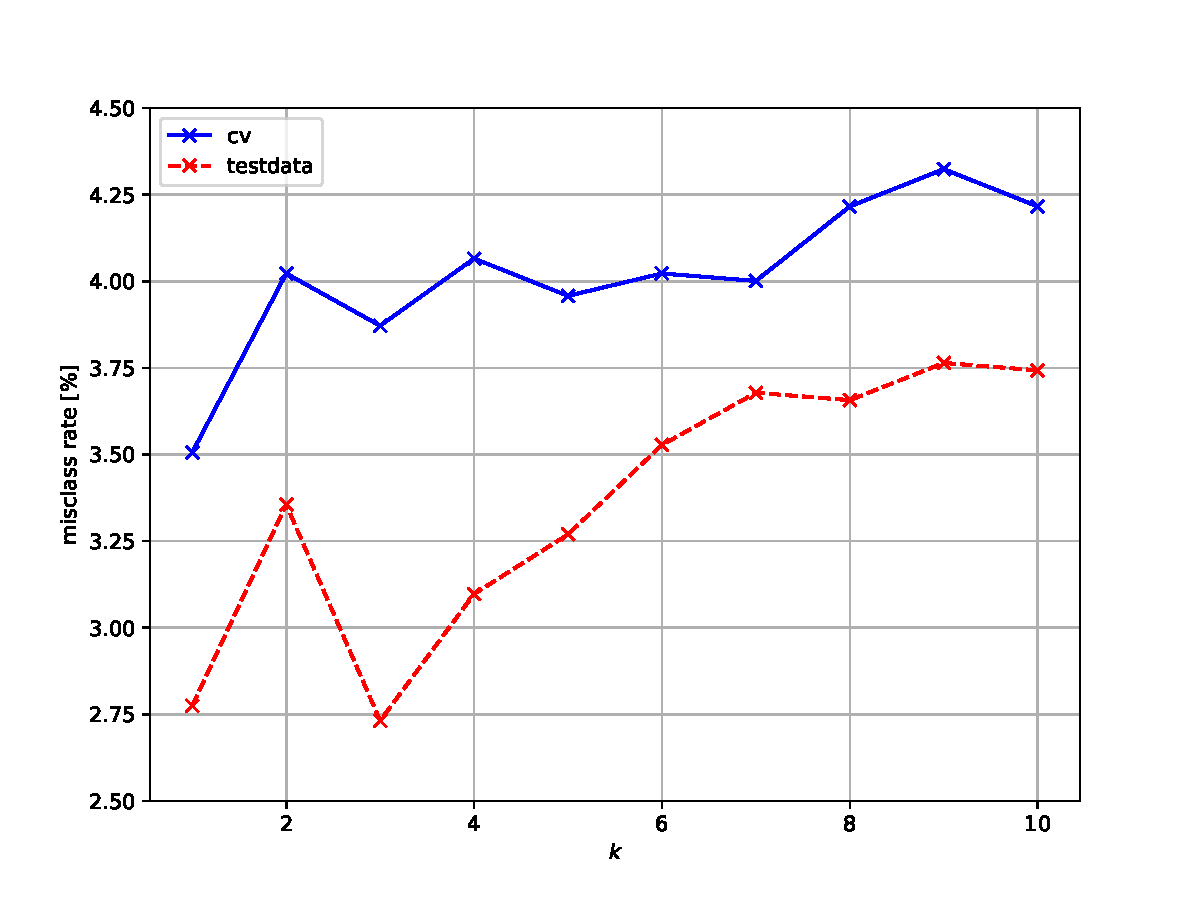
\includegraphics[width=1\textwidth]{fig_2.pdf}
        \caption{$k = 1, \dots, 10$ と誤識別率の関係}
        \label{fig:1}
      \end{figure}

      \quad

    \subsection{考察}

      実験結果から,今回の実験設定における,交差確認法により確認した最適な $k$ の値は,$k = 1$ であることがわかった.

      一方,ここで, $k$ とテストデータに対する誤識別率の関係を見ると,$k = 2$ で誤識別率は増加し,その後, $k=3$ で減少し,その後は再び増加している.

      これは,$k = 2$ では,学習データに過剰に適合してしまい,未知データに対する汎化性能が低下しているためであると考えられる.

      一方, $k \geq 4$ では,今度は学習データ全体の一般的な傾向を捉えすぎてしまい,学習データの細かな構造を無視してしまうことが原因であると考えられる.

  \section{課題2}
    
    \subsection{実験内容}

      画素値を特徴量とする代わりに,HOG 特徴を抽出し,これを特徴量とする.

      $k = 1, \dots, 10$ , HOG パラメータの CellSize を
      
      \[
      \begin{bmatrix}
      2 & 2
      \end{bmatrix}, \quad
      \begin{bmatrix}
      4 & 4
      \end{bmatrix}, \quad
      \begin{bmatrix}
      8 & 8
      \end{bmatrix}
      \]
      
      とするときの,最適な組合わせを求める.

    \subsection{実験結果}

      表 \ref{tab:2} は,CellSize を [2 2] としたときの,$k = 1, \dots, 10$ における誤識別率とサンプルあたり処理時間を示したものである.

      \begin{table}[p]
        \centering
        \caption{$k = 1, \dots, 10$ における誤識別率とサンプルあたり処理時間 (CellSize : [2 2])}
        \begin{tabular}{|c|c|c|c|}
          \hline
          $k$ & 誤識別率 (CV) [\%] & 誤識別率 (テストデータ) [\%] & サンプルあたりの処理時間 [s] \\
          \hline
          1  & 2.732 & 2.108 & 0.001403 \\
          2  & 3.097 & 2.560 & 0.001397 \\
          3  & 2.538 & 2.129 & 0.001392 \\
          4  & 2.839 & 2.237 & 0.001387 \\
          5  & 2.839 & 2.366 & 0.001397 \\
          6  & 2.925 & 2.323 & 0.001409 \\
          7  & 3.011 & 2.495 & 0.001397 \\
          8  & 3.097 & 2.495 & 0.001385 \\
          9  & 3.184 & 2.624 & 0.001398 \\
          10 & 3.227 & 2.689 & 0.001439 \\
          \hline
        \end{tabular}
        \label{tab:2}
      \end{table}

      表 \ref{tab:3} は,CellSize を [4 4] としたときの,$k = 1, \dots, 10$ における誤識別率とサンプルあたり処理時間を示したものである.

      \begin{table}[p]
        \centering
        \caption{$k = 1, \dots, 10$ における誤識別率とサンプルあたり処理時間 (CellSize : [4 4])}
        \begin{tabular}{|c|c|c|c|}
          \hline
          $k$ & 誤識別率 (CV) [\%] & 誤識別率 (テストデータ) [\%] & サンプルあたりの処理時間 [s] \\
          \hline
          1  & 2.818 & 2.366 & 0.000578 \\
          2  & 3.140 & 2.603 & 0.000576 \\
          3  & 2.818 & 2.302 & 0.000574 \\
          4  & 2.947 & 2.431 & 0.000576 \\
          5  & 2.753 & 2.581 & 0.000572 \\
          6  & 2.818 & 2.581 & 0.000580 \\
          7  & 3.076 & 2.732 & 0.000573 \\
          8  & 3.011 & 2.818 & 0.000581 \\
          9  & 3.011 & 2.925 & 0.000572 \\
          10 & 3.076 & 2.882 & 0.000572 \\
          \hline
        \end{tabular}
        \label{tab:3}
      \end{table}

      表 \ref{tab:4} は,CellSize を [8 8] としたときの,$k = 1, \dots, 10$ における誤識別率とサンプルあたり処理時間を示したものである.
      
      \begin{table}[p]
        \centering
        \caption{$k = 1, \dots, 10$ における誤識別率とサンプルあたり処理時間 (CellSize : [8 8])}
        \begin{tabular}{|c|c|c|c|}
          \hline
          $k$ & 誤識別率 (CV) [\%] & 誤識別率 (テストデータ) [\%] & サンプルあたりの処理時間 [s] \\
          \hline
          1  & 7.378 & 6.776 & 0.000410 \\
          2  & 7.830 & 7.120 & 0.000414 \\
          3  & 6.797 & 6.302 & 0.000411 \\
          4  & 6.819 & 6.647 & 0.000412 \\
          5  & 6.926 & 6.539 & 0.000415 \\
          6  & 7.292 & 6.453 & 0.000412 \\
          7  & 7.184 & 6.647 & 0.000414 \\
          8  & 7.227 & 6.776 & 0.000414 \\
          9  & 7.249 & 6.883 & 0.000414 \\
          10 & 7.335 & 6.840 & 0.000417 \\
          \hline
        \end{tabular}
        \label{tab:4}
      \end{table}      

    \subsection{考察}

      実験結果から,HOG パラメータの CellSize = [2 2] で,$k = 3$ のとき,誤識別率 (CV) が最も低くなり,最適な組合わせであると言える.

      CellSize が小さいとき,特徴量の次元が大きくなるため,計算量が増加するが,一方で,特徴量の粒度が細かくなるため,特徴量の表現力が向上する.ただし,過学習に注意する必要がある.

      一方,CellSize が大きいとき,特徴量の次元が小さくなるため,計算量が減少するが,一方で,特徴量の粒度が荒くなるため,特徴量の表現力が低下する.

      今回の実験においては,CellSize = [2 2] が最適であると言える.
      
  \section{まとめと感想}

    本実験では,k-最近傍法を用いて手書き数字の識別を行った.

    また,HOG 特徴を用いて,最適な $k$ と HOG パラメータの CellSize を求める実験を行った.

    今回の実験では,k-最近傍法の原理を理解するとともに,HOG 特徴を用いた画像認識の基礎を学ぶことができた.

    機械学習の仕組みは,つきつめるとシンプルな原理に基づいているが,その上で,計算量の改善や特徴量の選択など,人類のたくさんの工夫によって支えられているのが興味深いと感じた.

    今後は,畳み込みニューラルネットワーク (CNN) などのより高度な画像認識手法についても学びたいと考える.

\end{document}
